I Logical view vil man kunne finde pakke opdelinger af de forskellige software dele. Derudover er der en illustrering af hvordan brugerens grænseflade hænger sammen og beskrivelser af nogle kritiske CSS-hovedenheds klasser.

\subsection{Bruger grænseflade (JC)}

\begin{figure}[!htb]
     {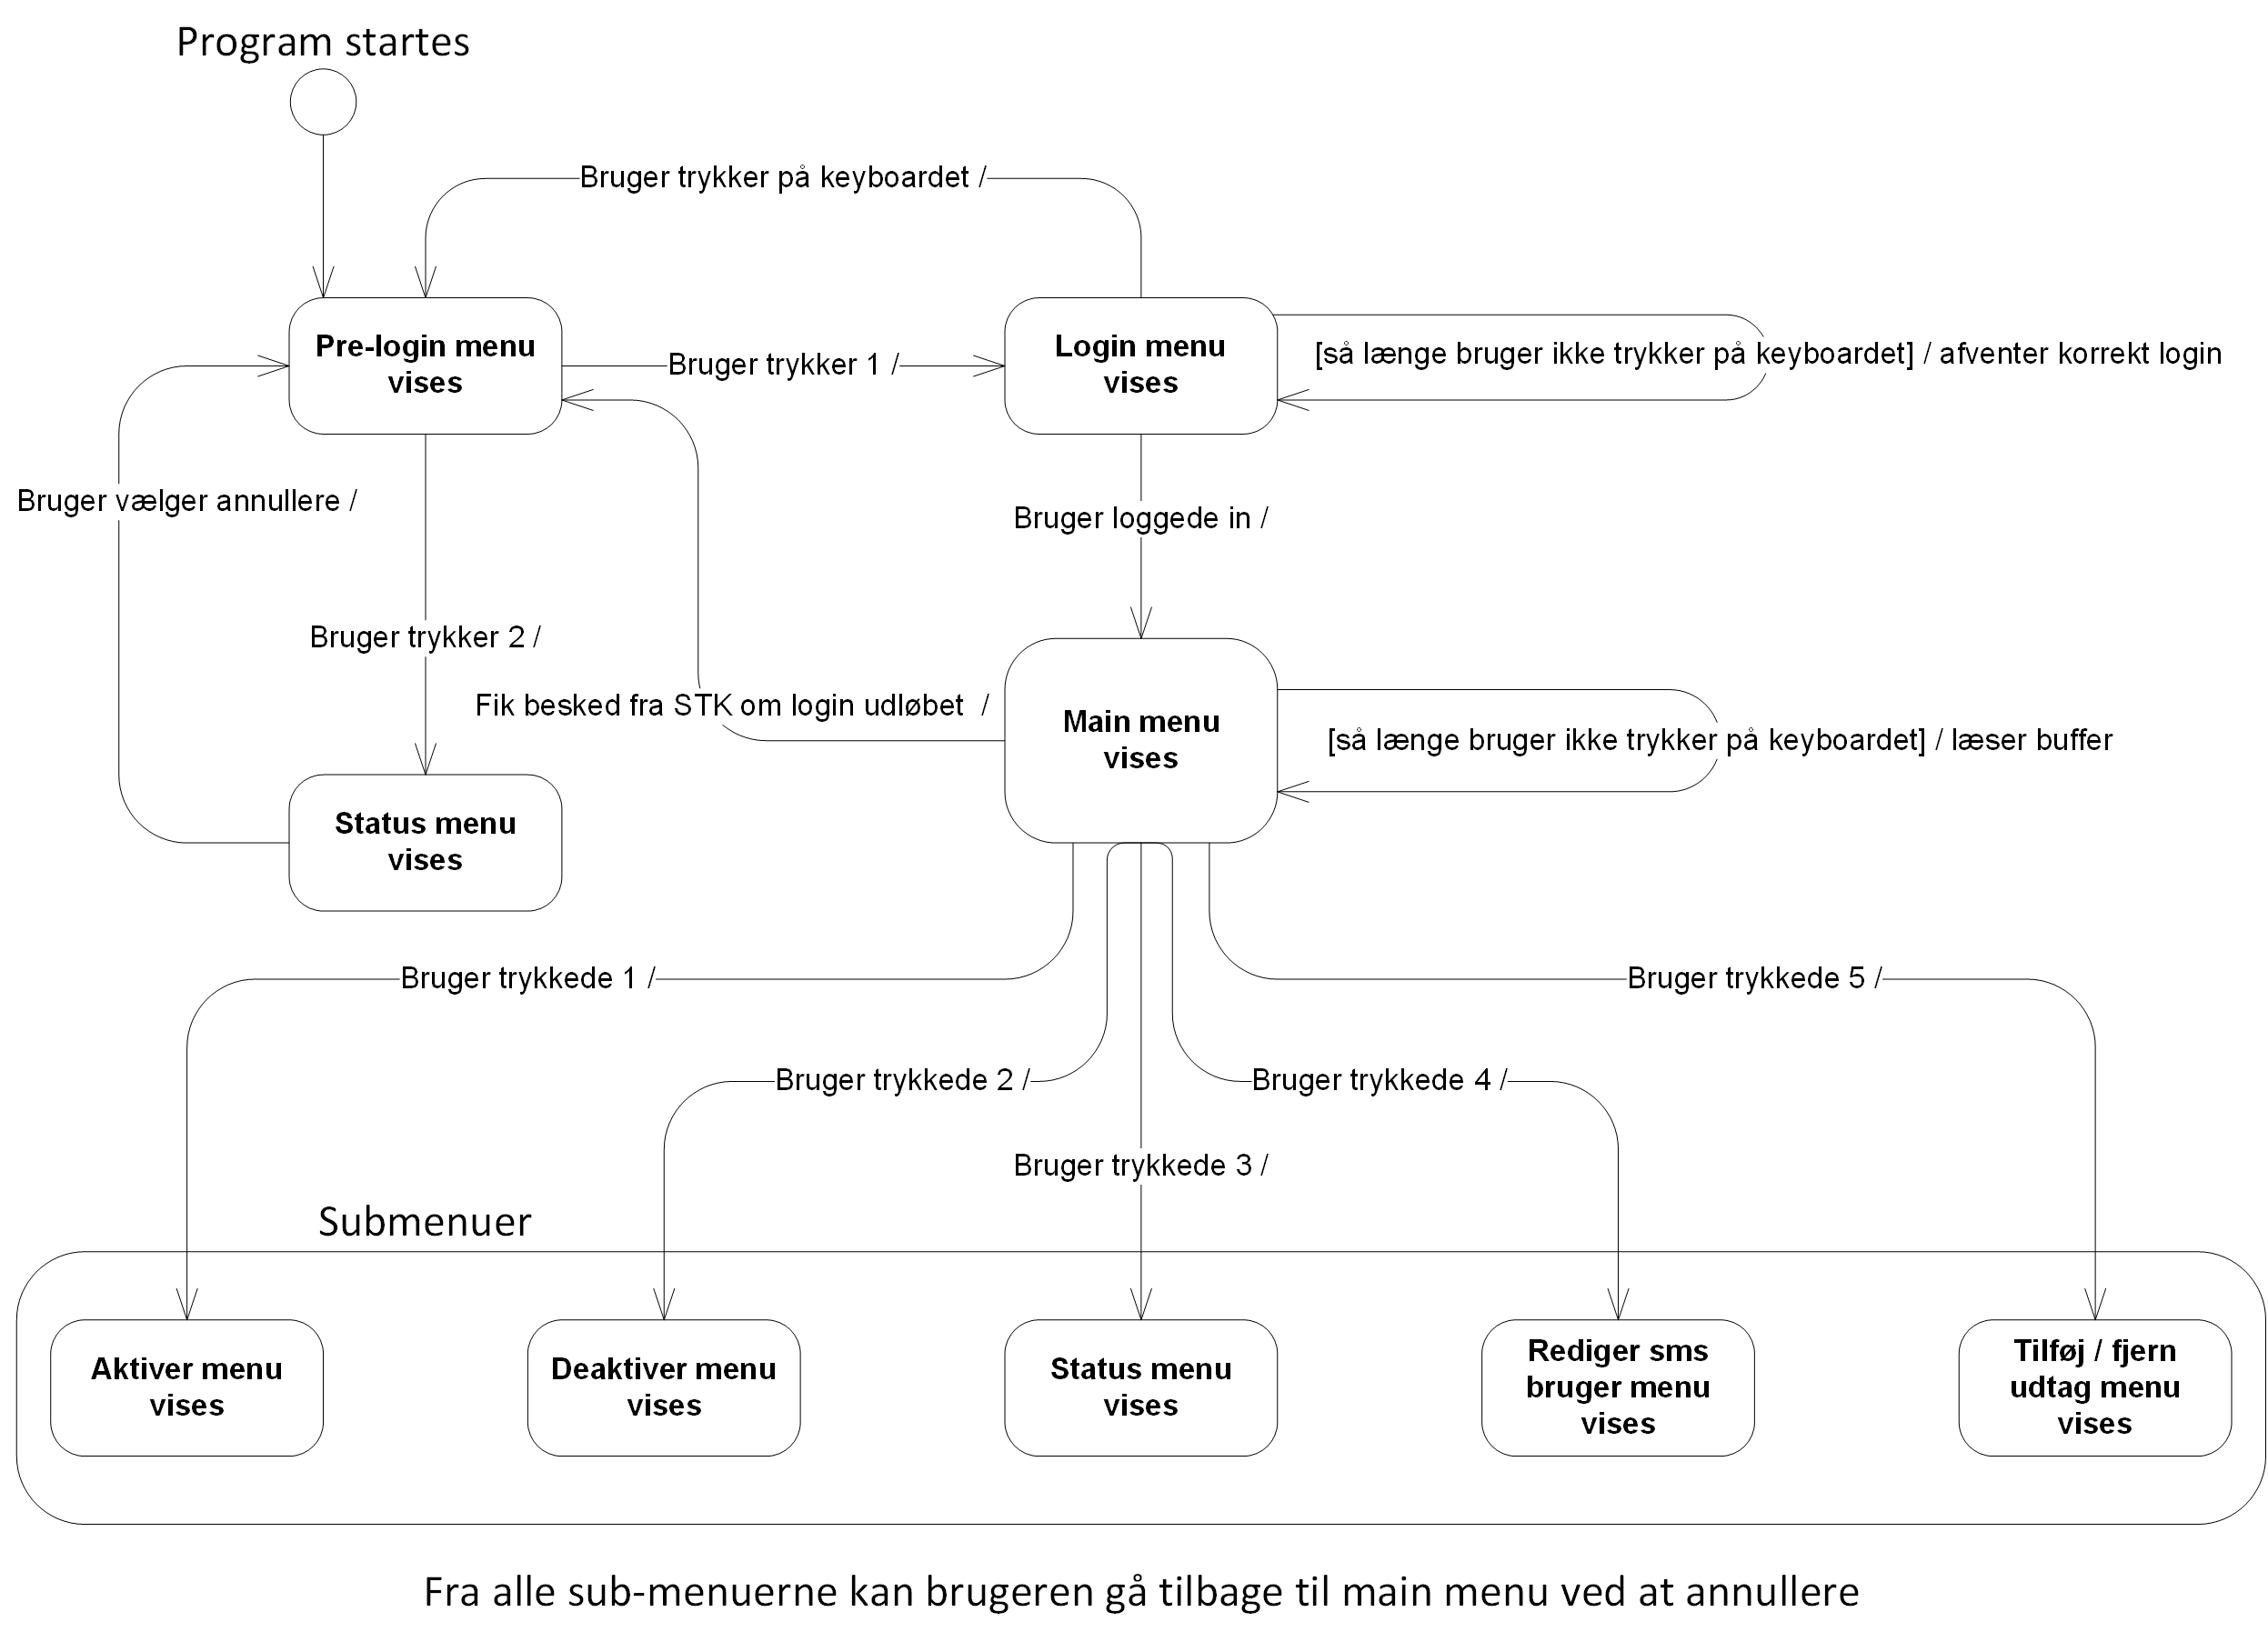
\includegraphics[width=\textwidth]{billeder/uml/state_machine_main}}
     \caption{State machine diagram over forløbet fra PC start til menuer.}
     \label{fig:State_machine_pc}
\end{figure}

Diagrammet ovenfor skal illustrere hvordan forløbet er fra PC opstart. Hvor man møder Pre-login menuen som kun giver en mulighed for at få vist login menu eller vis status menu. Efter der er logget ind vil den stå og føle på input bufferen, på den port hvor PC'en er forbundet med CSS hovedenheden. Det gør den for at en evt. babyalarm kan afbryde forløbet og blive sendt. Desuden kan CSS-hovedenheden give besked om at der ikke længere er logget ind, hvilket sender brugeren til pre-login menuen igen.

\medskip

Når brugeren så trykker på en tast og trykker enter vil han blive sendt til en af de 5 menuer. Dog stadig under forudsætning af at han valgte en værdi imellem 1-5 for den pågældende menu. Ved forkert tast sker der ingenting. Fra hver af de 5 sub-menuer har Brugeren mulighed for at annullere og komme tilbage til main menuen. Dette gør denne ved at taste 27 og enter.


\clearpage

\subsection{Software packages (JC)}

\begin{figure}[!htb]
     {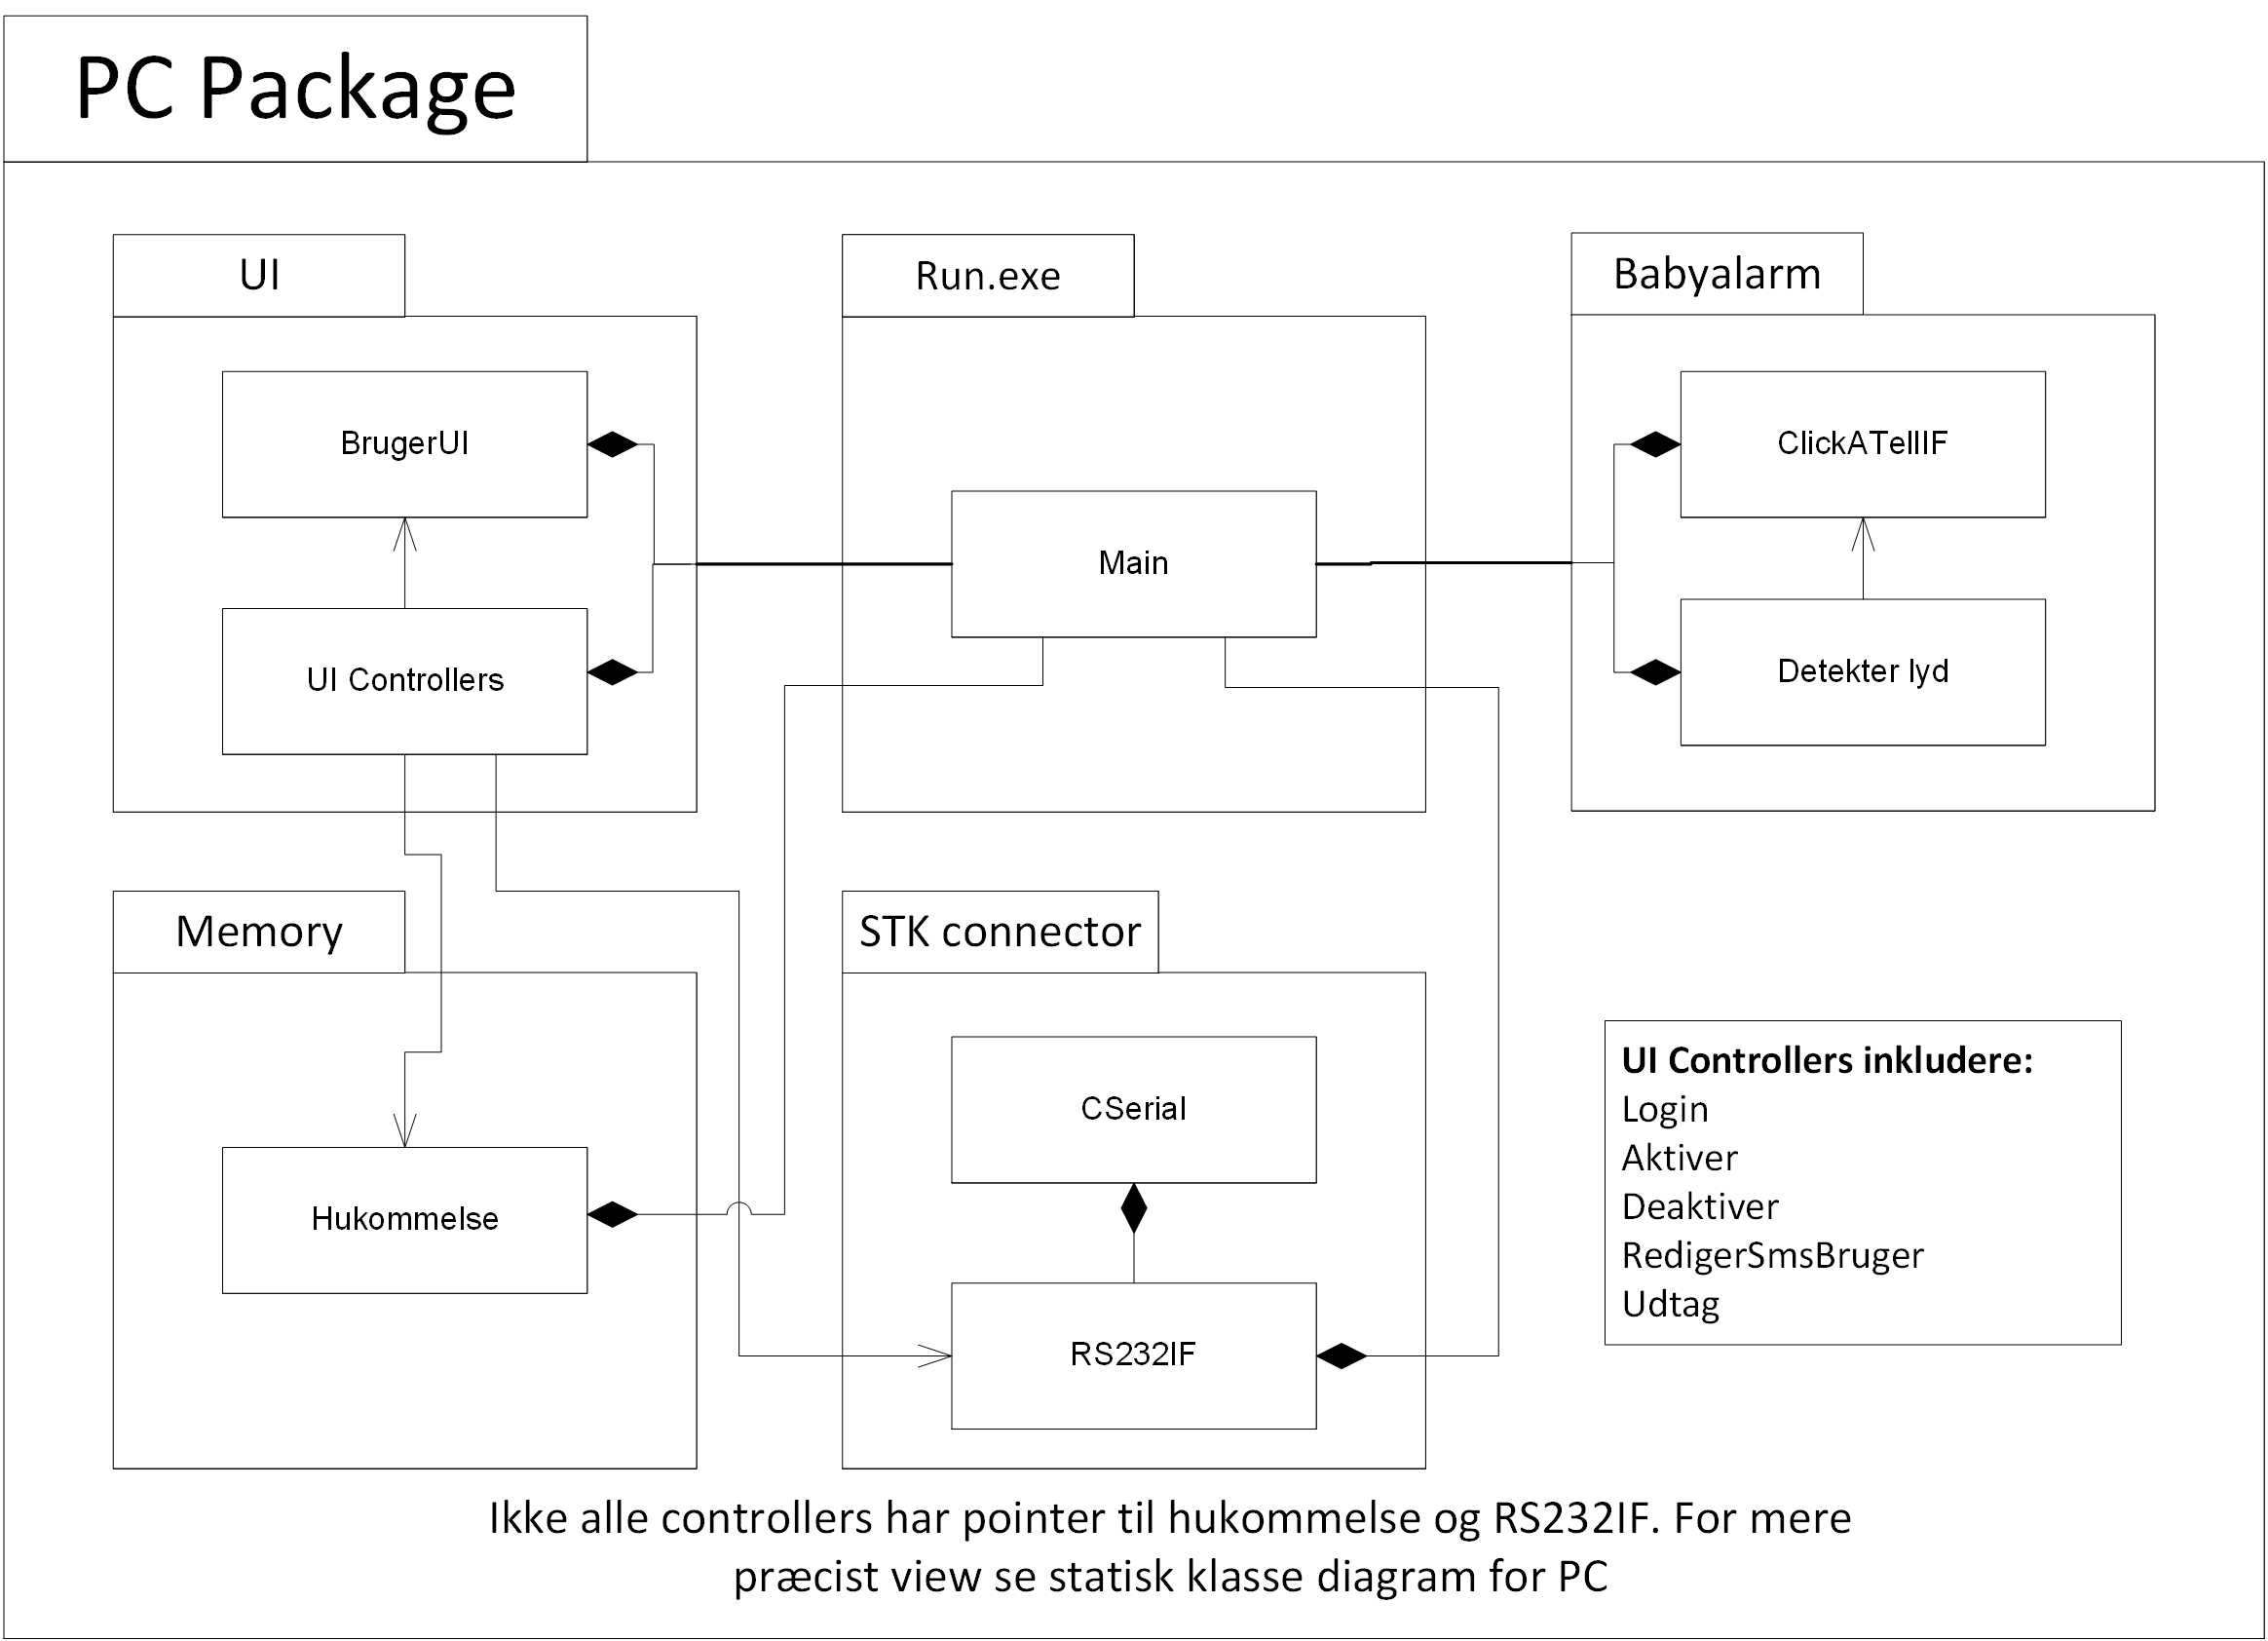
\includegraphics[width=\textwidth]{billeder/uml/logical_view_pc}}
     \caption{Logical view: PC package}
     \label{fig:PC_package}
\end{figure}

Figuren ovenfor viser de forskellige pakker man kan indlede PC klasserne i. Alle controllers som har UI pointers er smidt i UI pakken sammen med BrugerUI. STK Connector pakken indeholder RS232IF og så har den et CSerial \footnote{CSerial klassen findes på http://tinyurl.com/mvzmcep. Kildekode og URL genvej findes på CD'en i Reference mappen. Tom Archer and Rick Leinecker, år 1999. [27.05.2014] } objekt som er en klasse der har de 5 mest basale metoder til at sende og læse på en seriel port.


\clearpage

\begin{figure}[!htb]
     {\includegraphics[width=\textwidth]{billeder/uml/logical_view_CSS_Hovedenhed}}
     \caption{Logical view: CSS Hovedenhed package}
     \label{fig:CSS_Hovedenhed_package}
\end{figure}

Figuren ovenfor viser de forskellige pakker man kan inddele CSS hovedenheds klasser i.

\clearpage

\begin{figure}[!htb]
     {\includegraphics[width=\textwidth]{billeder/uml/logical_view_CSS_Udtag}}
     \caption{Logical view: CSS Udtag package}
     \label{fig:CSS_Udtag_package}
\end{figure}

Figuren ovenfor viser de forskellige pakker man kan inddele CSS udtagets klasser i. 

\clearpage

% CircBuffer
\subsection{Klasse CircBuffer (BS)}
Efter som X10 kommunikationen er meget langsom (50 bits/s) bruges en buffer til at holde på kommandoerne ind til de er klar til at blive afsendt. Dette er CircBuffer klassens opgave.
Denne er udformet som en cirkulær buffer som kan holde 2 fulde kommandoer. Bemærk at i følge X10-protokollen skal alle kommandoer afsendes to gange. Så der er plads til 4 kommandoer, hvor to af dem altid er de samme.

Klassen er bygget til selv at holde styr på hvilket bit der skal sendes næste gang. Dette forenkler brugen væsentligt, da udtagning af data fra bufferen sker fra en interrupt service rutine (ISR). Denne rutine er beskrevet i detaljer senere.

Alle kommandoer termineres med '\textbackslash 0' karakteren. 

% X10IF klasse design
\subsection{Klasse X10IF (BS)}
En af de kritiske og avancerede klasser er X10IF klasserne på hhv. CSS-hovedenheden og X10 Udtaget. I designfasen er der udviklet sekvensdiagrammer som beskriver nogle af metoderne og sammenspillet til andre klasser.

Funktionaliteten for metoden sendKommando() i X10IF klassen, på CSS-hovedenheden, har som ansvar at afsende en fuld X10-kommando, iht. protokollen, ud fra en parameter formateret som vist i tabel \ref{table:X10_sendKommando_format}.

\begin{table}[h]
	\caption{Parameter opbygning til sendKommando() metoden i X10IF}
	\centering
	\begin{tabular}{|c|c|c|}
		\hline 
		\textbf{Byte} & 0 & 1..4 \\ \hline
		\textbf{Data} & Kommando & Adresse \\ 
		\hline 
	\end{tabular} 
	\label{table:X10_sendKommando_format}
\end{table}

Metoden skal først omskrive den modtagende kommando til en X10 bit streng. Her efter indsættes alle bit's i en buffer, hvorfra de afsendes når der detekteres et zero cross. 
Sekvensen er vist i figur \ref{fig:X10_sendKommando_sd}.

\begin{figure}[!htb]
     {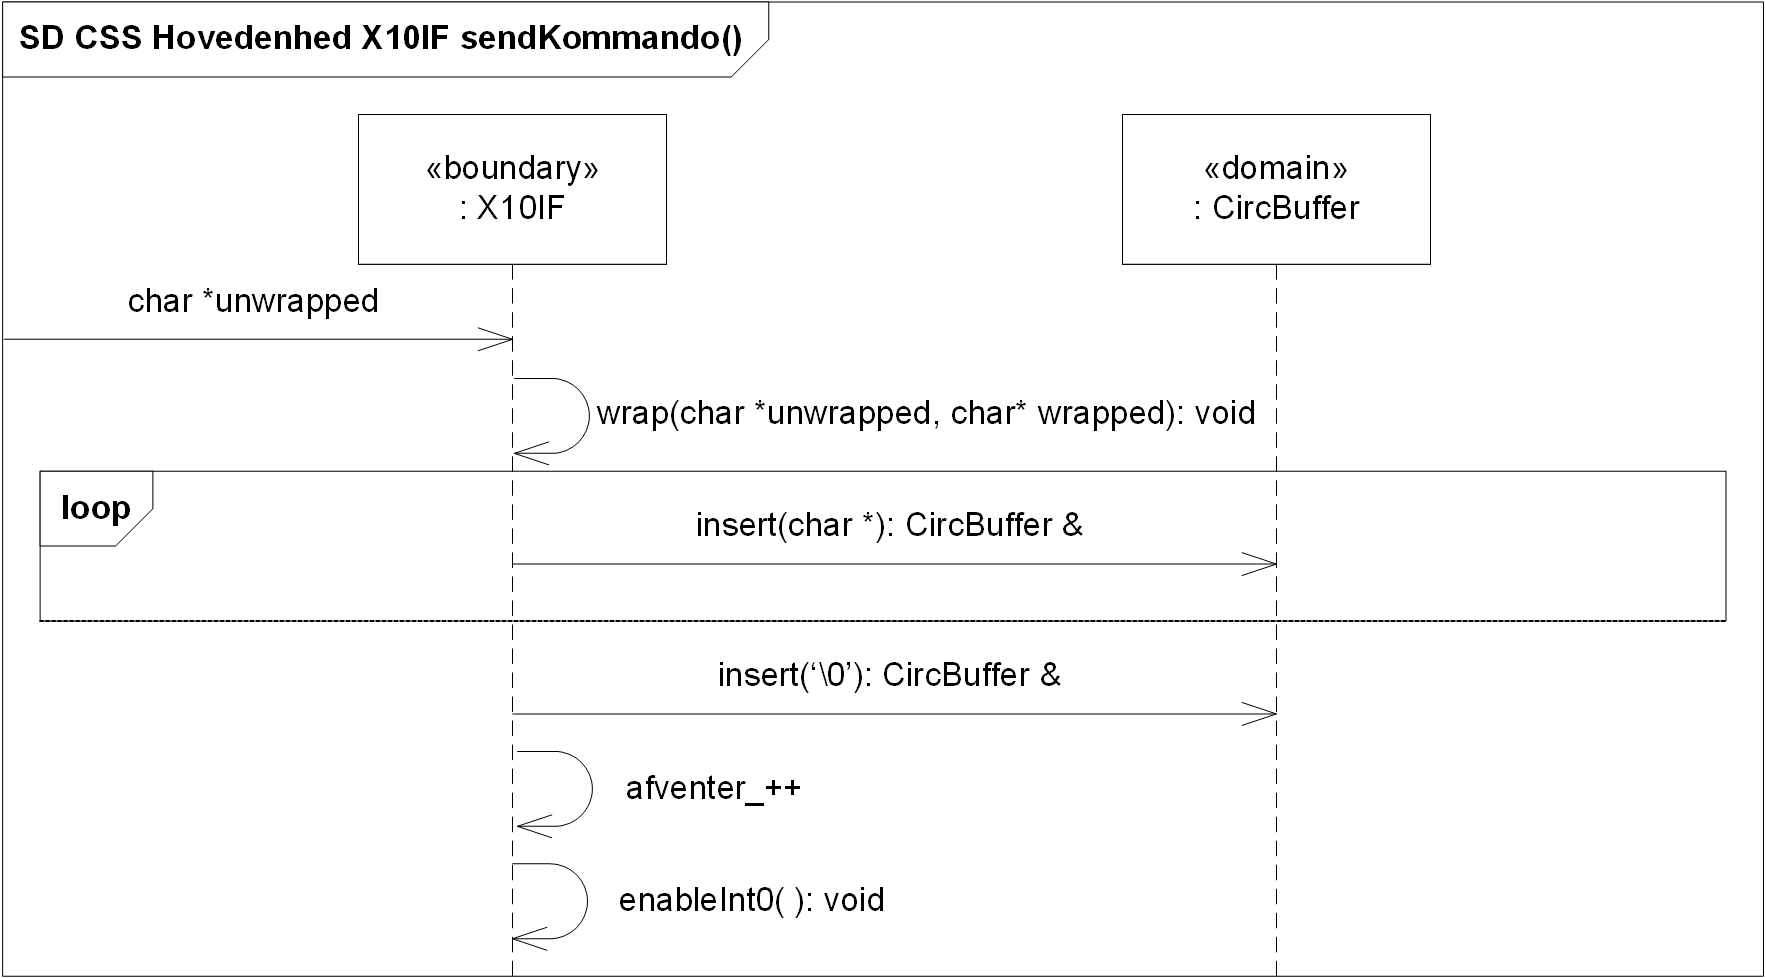
\includegraphics[width=\textwidth]{billeder/uml/CSS_X10IF_sendKommando_SD}}
     \caption{Sekvensdiagram for metoden sendKommando() i X10IF klassen på CSS hovedenheden}
     \label{fig:X10_sendKommando_sd}
\end{figure}

% ZeroCrossInt ISR
\subsection{ZeroCrossInt funktion (BS)}
I tilfælde af et interrupt signal på INT0 benet på CSS-hovedenheden køres en bestemt funktion i microcontrolleren. Dette er kaldet en ISR. Forløbet for denne er beskrevet i sekvensdiagrammet på figur \ref{fig:ZeroCrossISR}.
Først kontrollerer den om der er nogle kommandoer i kø. Der efter henter den det næste bit der skal afsendes fra bufferen. Ud fra værdien bestemmer den om der skal tændes for 120 kHz frekvensen i timeren. Når en kommando er helt sendt nedskriver den køen og hvis køen er tom slår den interruptet fra.

\begin{figure}[!htb]
     {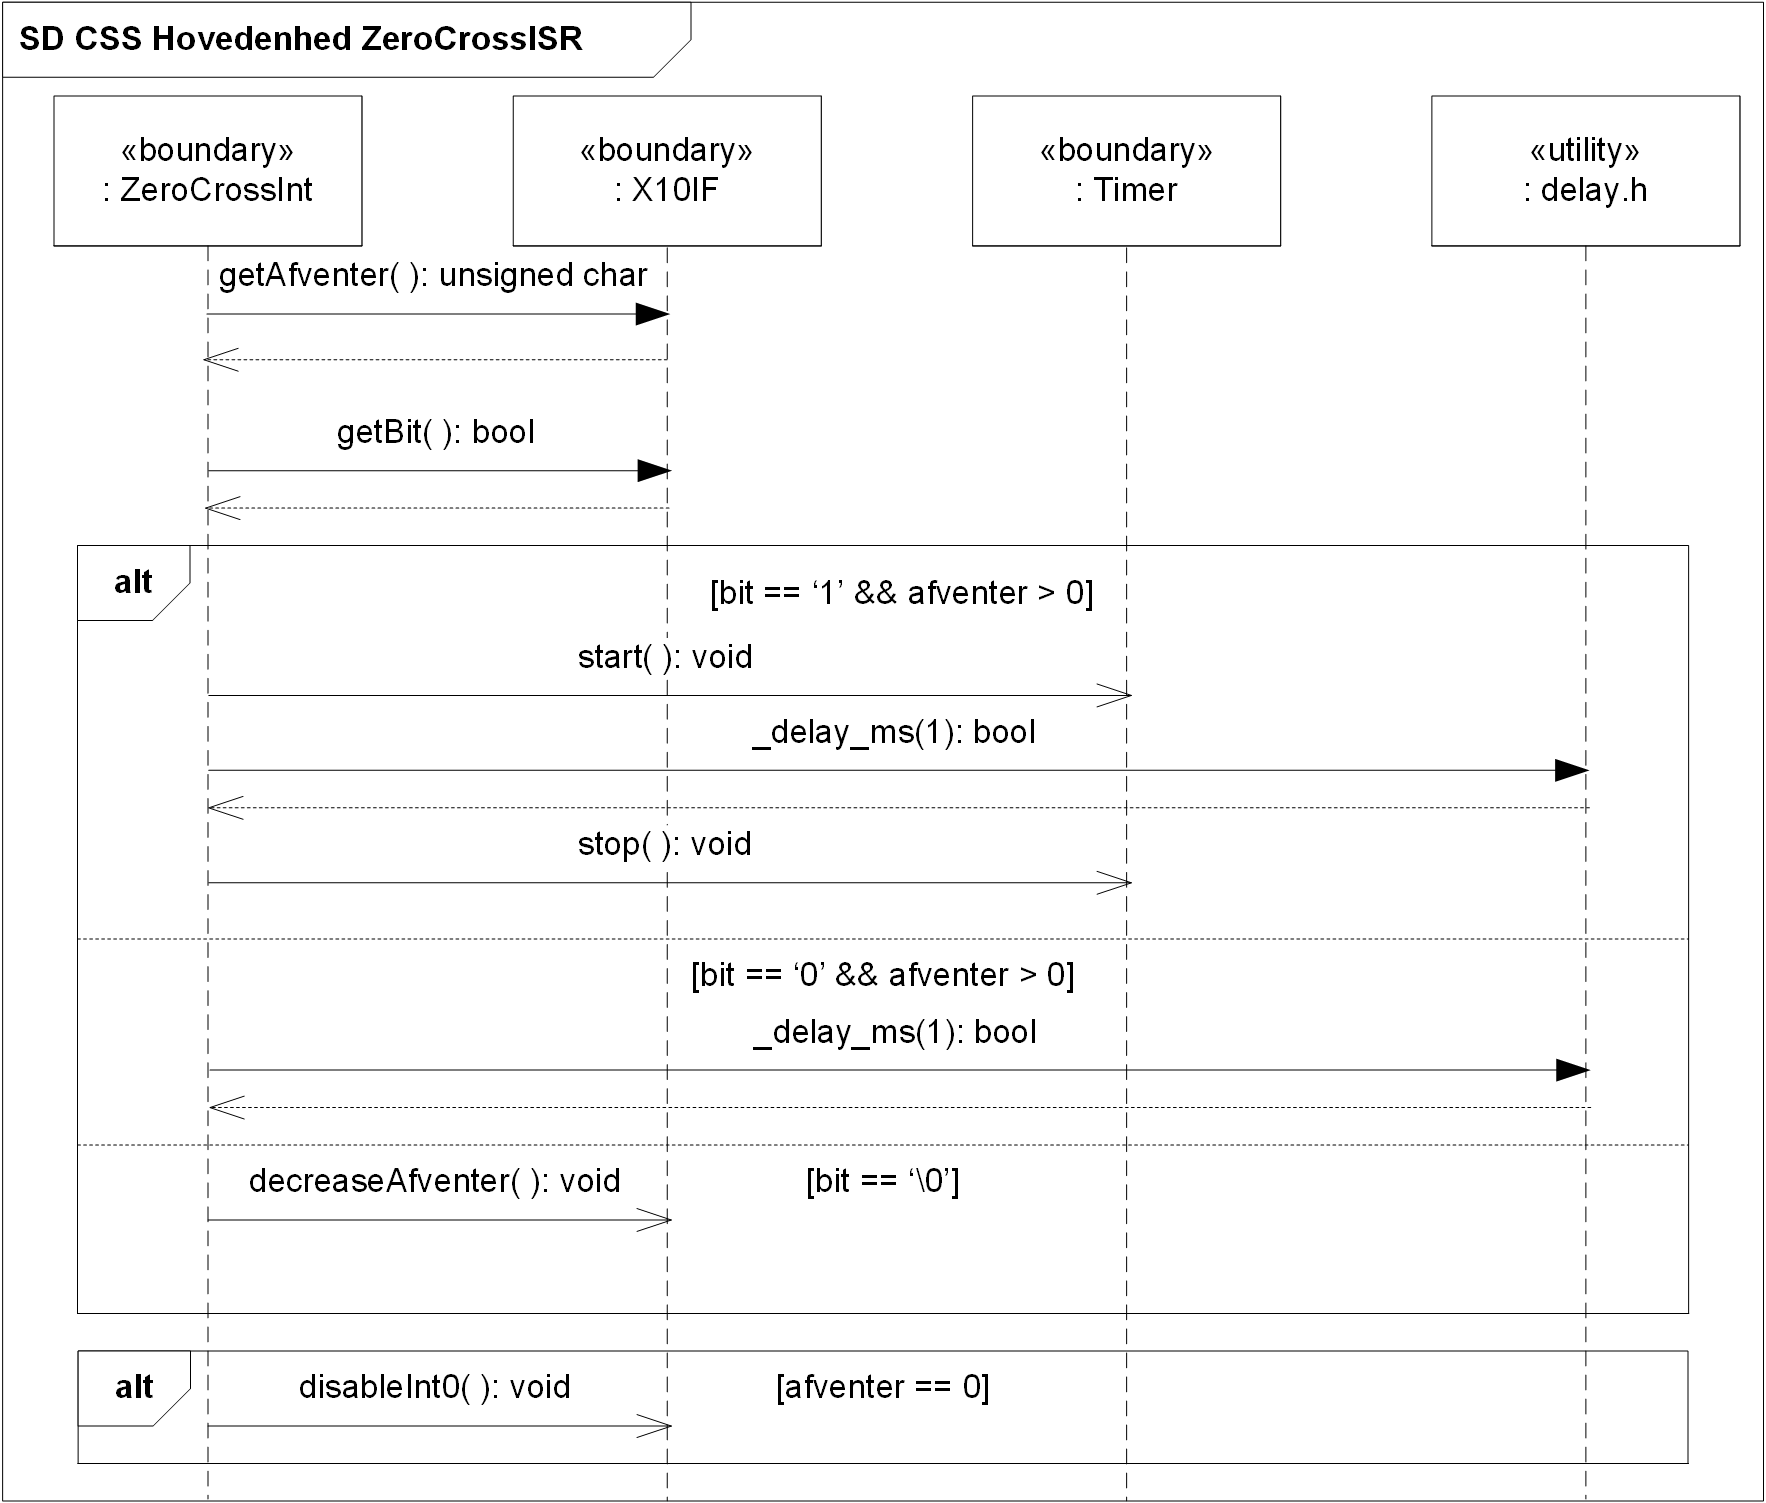
\includegraphics[width=\textwidth]{billeder/uml/CSS_ZeroCrossInt_SD}}
     \caption{Sekvensdiagram for INT0 ISR på CSS hovedenheden}
     \label{fig:ZeroCrossISR}
\end{figure}

% ClickATell
\subsection{Klasse ClickATell (BS)}
For at kunne afsende SMSer i tilfælde af babyalarm bruges en API som kan afsende beskeder via internettet.
ClickATell\textsuperscript{\circledR}\footnote{Online SMS service: http://www.clickatell.com/} er en online service som kan afsende SMSer til et valgfrit telefonnummer ved at kalde en URL adresse.
Ved at bruge Microsoft Windows Shell API\footnote{Microsoft MSDN: http://tinyurl.com/d99m9dz} er det muligt at starte applikationer fra Windows miljøet. Dette bruges til at starte et Internet Explorer-browservindue med en predefineret URL adresse som skaber forbindelse til ClickATell\textsuperscript{\circledR} APIen. 

% Klasse X10IF (udtag)
\subsection{Klasse X10IF (udtag)}
Denne klasse modtager og bearbejder X10 signalet, i tilfælde af interrupt signal på INT1 benet køres en interrupt service rutinen som kigger efter om der er et højt- (logisk '1') eller lavt- (logisk '0') signal input på PD5 benet. Det modtaget bit bliver sendt til insertX10bit funktionen som lager de modtaget bit løbende i et char array kaldet X10Array\_, funktion kontroller løbende de fire første pladser i arrayet for STX kommandoen, som er X10 signalets start kommando, når funktionen detekter at der er modtaget en STX kommando lager den de næste 24 bit der bliver modtaget i array'et som derefter bliver sendt til funktionen unwrapX10Array. unwrapX10Array metoden dekoder den modtaget X10 formateret kommando og adresse. Og sender herefter adressen via den matchet kommando, via funktionen aktiver eller deaktiver alt efter hvilken match der er lavet, til den tilhørende controller.
Sekvensen for unwrapX10Array kan ses i figur \ref{fig:X10-Udtag_unwrapX10Array_SD}.

\begin{figure}[!htb]
     {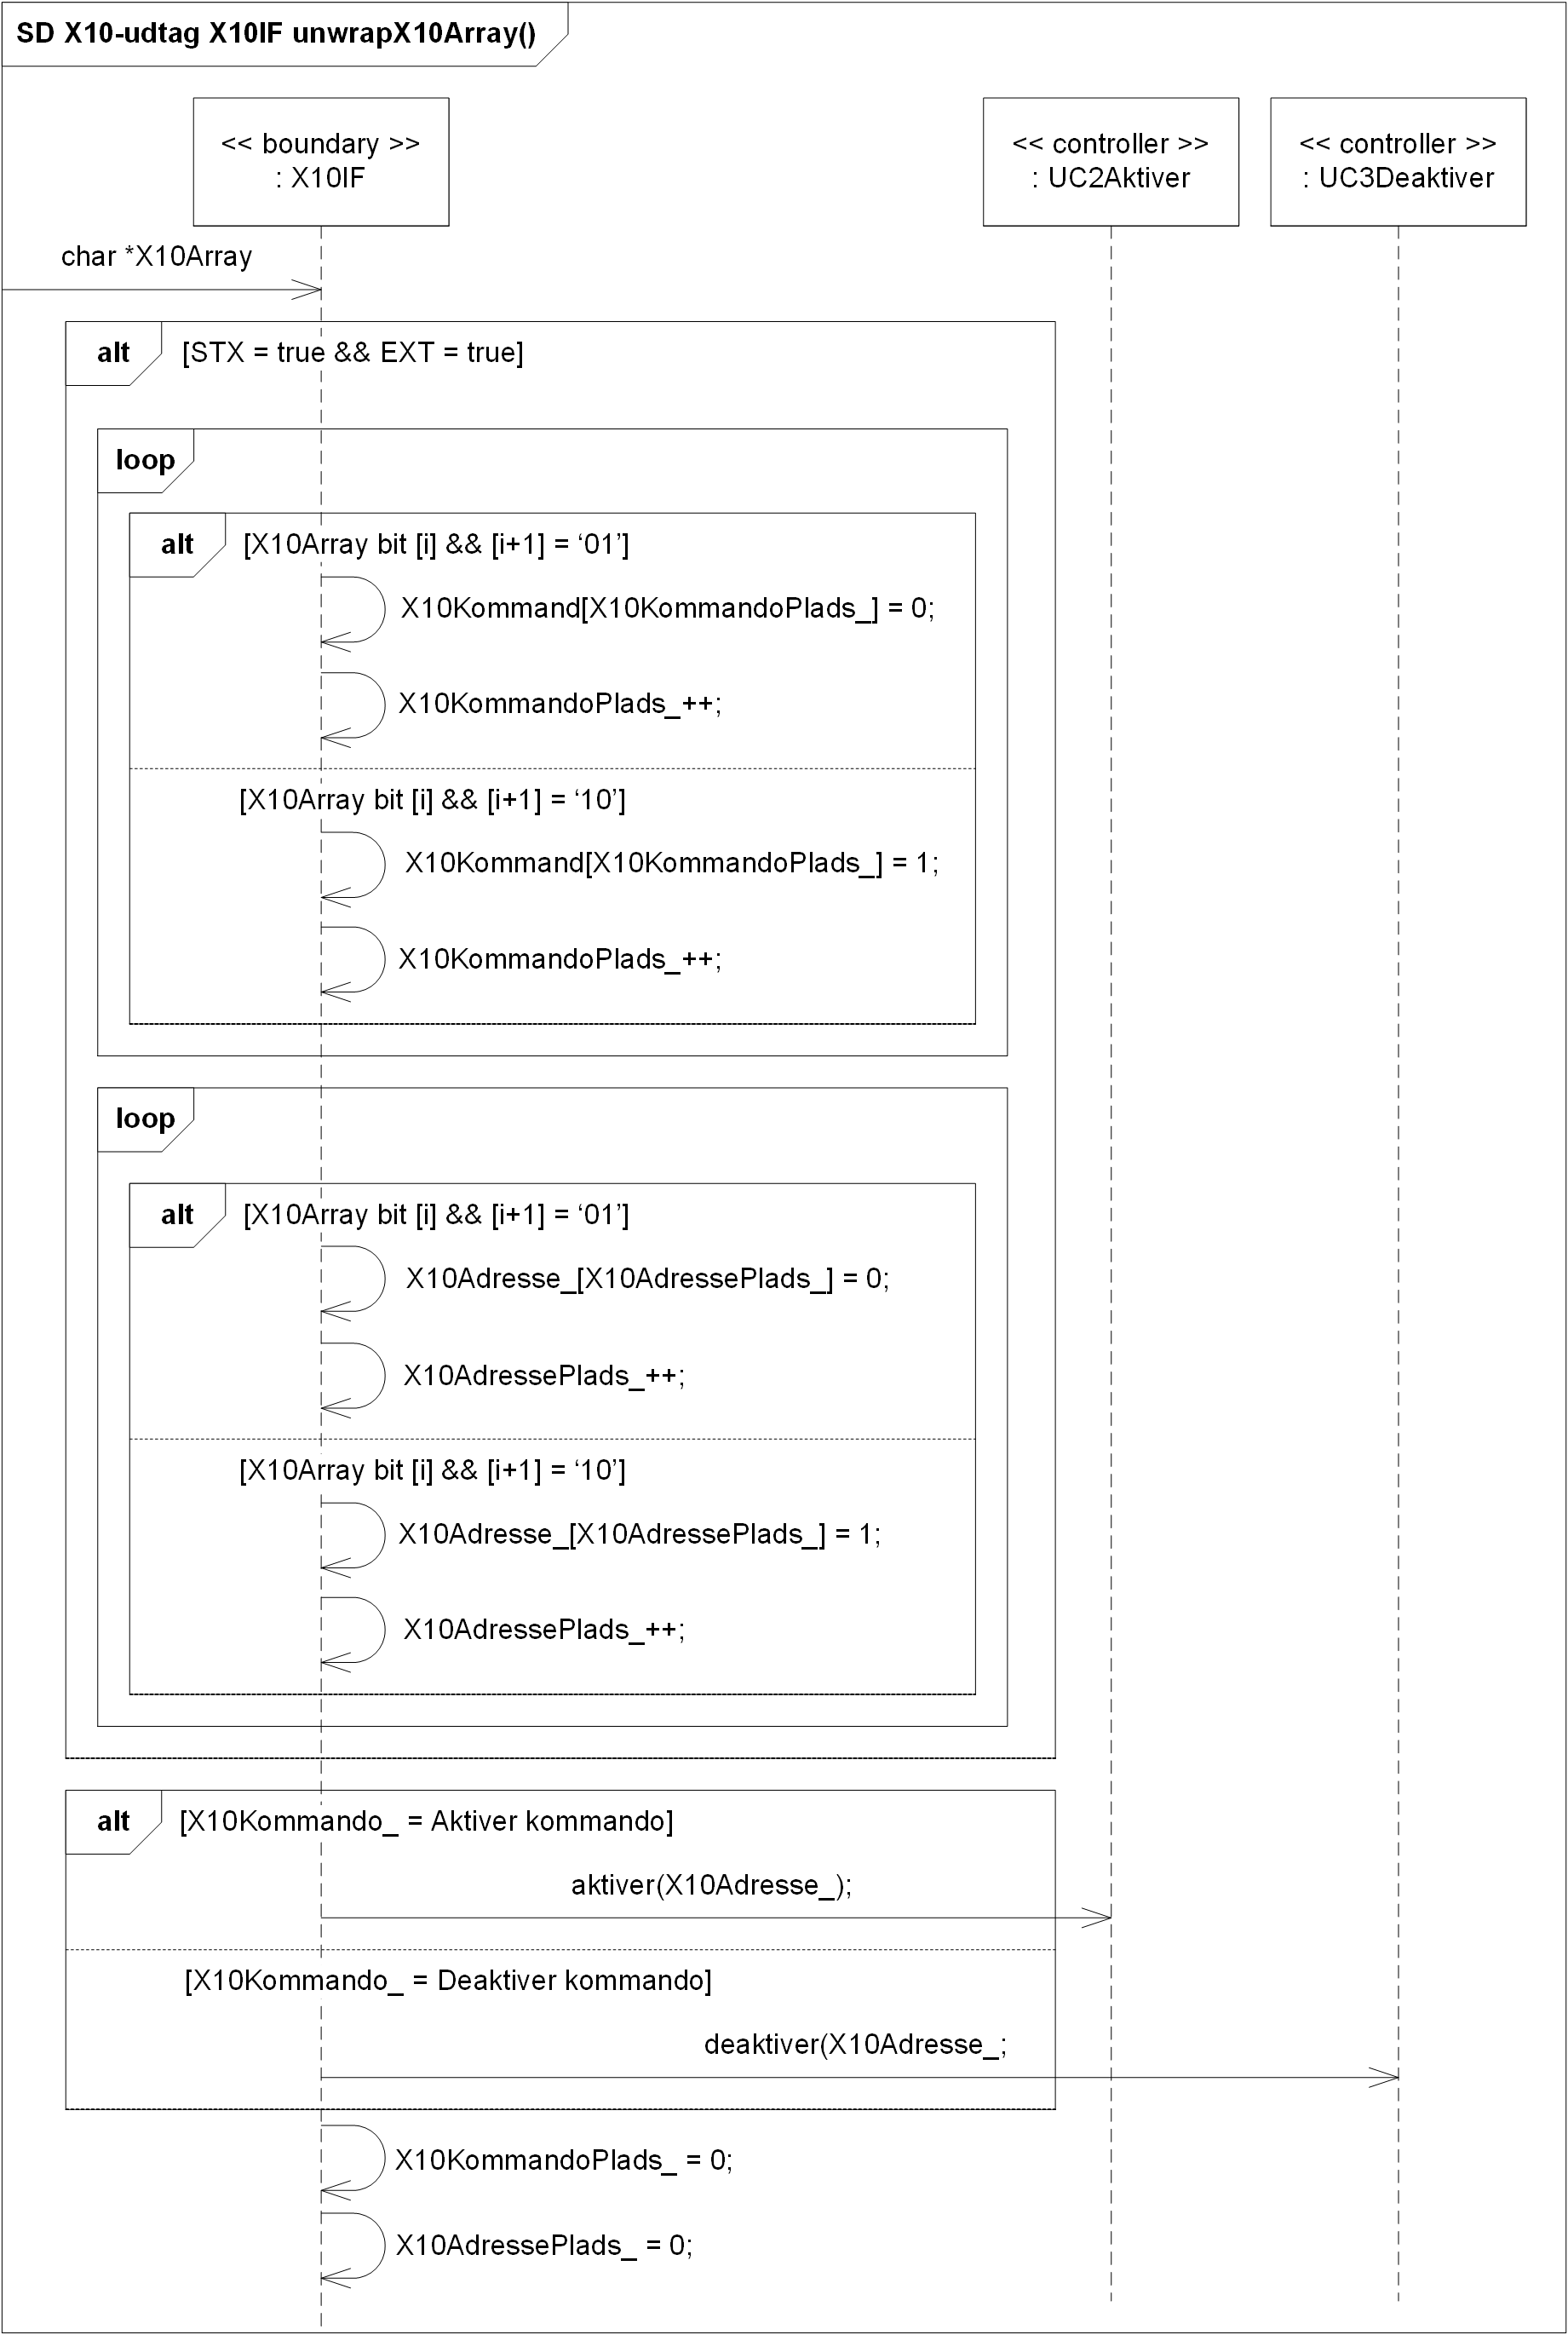
\includegraphics[width=\textwidth]{billeder/uml/X10-Udtag_unwrapX10Array_SD}}
     \caption{Sekvensdiagram for metoden unwrapX10Array() i X10IF klassen på X10-udtaget}
     \label{fig:X10-Udtag_unwrapX10Array_SD}
\end{figure}
